\chapter{Tablas de Dispersión}
Las \textbf{tablas de dispersión} o \textbf{tablas hash} son aquellas que almacenan elementos de un conjunto mediante el uso de una \textbf{función hash}, que dado un elemento devuelve su posición exacta en la tabla que se almacena.

El tiempo de búsqueda de dicho elemento es de coste \(O(1)\), ya que tenemos acceso directo a dichos elementos de un conjunto, esto es así ya que el tiempo que se tarda en calcular la función hash es constante.


Una idea propuesta es que cada elemento que se almacena se compone de una clave, estas claves son números entero y dependen del tamaño del vector \(M\), donde el rango de las mismas es [\(0, M-1\)], por tanto, si queremos acceder al elemento `i', será de la manera \(h(i) = i\).

También podemos encontrar problemas con dicha idea, ya que pueden que no estén acotadas (demasiado grandes para el tamaño del vector), la claves no son de tipo entero..

\section{Funciones Hash}
Las \textbf{funciones hash} transforman una clave de un cierto tipo (número, cadena, fecha, etc) en una \textbf{dirección} o \textbf{índice} de la propia tabla hash, \(h: C\) →\([0, M-1]\), donde \(C\) es el conjunto de posibles claves.

Debido a esto encontramos las \textbf{colisiones} entre claves que se produce cuando a dos claves diferentes le corresponden como resultado el mismo valor de función hash. Si esto ocurre decimos que ambas son \textbf{claves sinónimas}.

Por tanto, una \textbf{función hash perfecta} es aquella que no produce ninguna colisión entre todas las claves posibles \(C \leq M\) (el cardinal de C es menor al tamaño del vector).

Pero esto es algo teórico, ya que en la práctica el número de claves posibles es mayor al tamaño del vector \(C > M\), por tanto, es inevitable que se produzcan colisiones entre claves.

Propiedades que encontramos en las buenas funciones hash:
\begin{itemize}
  \item Eficiencia temporal → Rapida de calcular.
  \item Eficiencia espacial → Función \underbar{sobreyectiva}(todas las posciones de la tabla corresponden a una clave).
  \item Distribución uniforme → Reduce la posibilidad de colisiones entre claves.
\end{itemize}

Esto no es algo sencillo y presenta algunas dificultades.

Una función hash la podemos construir en dos partes:
\begin{enumerate}
  \item Definir una función que hash \textbf{H(x)} que transformen las claves a números enteros.
  \item Trasladar cualquier número a una dirección obtenida mediante el calculo de su módulo respecto al tamaño del vector → \(h(x)= H(x)\ mod\ M\).
\end{enumerate}

\section{Resolución de colisiones}
Como hemos comentado anteriormente, en la práctica las colisiones son algo \textit{inevitable}, para hacerles frente podemos definir diferentes tipos de hashings (hashing cerrado, abierto o encadenamiento mezclado).

Tenemos que diferenciar que la \textbf{sinonímia} \(\rightarrow\) \textbf{colisión}, pero la \textbf{colisión} \(\nrightarrow\) \textbf{sinonímia}.

\section{Hashing Cerrado}
Cuando se produce una colisión, se busca una nueva posción libre en la tabla.
Aquí encontramos una \textbf{secuencia de exploración} para poder localizar dicha posición libre de la tabla.
Esto se realiza mediante una serie de \textbf{M funciones hash} \(\{h_{0},h_{1},h_{2},...,h_{M-1}\}\), donde \(h_{0}\) es la función hash original.

\subsection*{Exploración lineal}
Tenemos que \(h_i = (h_0\ +\ i\ *\ \alpha) \ mod\ M\), donde la distancia entre celdas \(\alpha \in \mathbb{N}\)  y es primo relativo con \(M\).

Este tipo de hash produce \textbf{agrupamientos primarios} → posiciones ocupadas \(\alpha = 1\), esto aumenta el tiempo de posteriores colisiones debido a que se puede producir un gran bloque de claves, lo que denominamos \textbf{degradación muy rápida de la eficiencia de las operaciones}. 

\subsection*{Exploración cuadrática}
Ahora tenemos \(h_i = (h_0\ +\ i^2)\ mod\ M\), ahora la distancia entre celdas aumenta exponencialmente.

Ahora encontramos que se producen \textbf{agrupamientos secundarios} de claves sinónimas debido a que la secuencia de exploración desde \(h_0 \)(+1, +4, +9, +16,..), además estos agrupamientos secundarios se entrelanzan pero no se unen para formar otros mayores, es decir, son menos perjudiciales para la eficiencia temporal que los agrupamientos primarios.

\subsection*{Exploración aleatoria}
Este es otro tipo de hahing cerrado, donde \(h_i = (h_0\ +\ x_i)\ mod\ M\), donde \(x_i\) se obtiene mediante una generador de números aleatorios (GNA).

El GNA tiene que generar dichos números cuya distribución debe de ser uniforme, es decir, que tengan la misma probabilidad para permitir recorrer todas las posciones.

Este tipo de hashing cerrado evita los agrupamientos de claves sinónimas si usamos una semilla diferente para cada clave, de modo que tendremos secuencias de exploración diferentes.

\subsection*{Hashing doble}
En este tipo de hashing encontramos una segunda función hash \(h^`\), quedando la función hash como \(h_i = (h_0\ +\ i\ *\ h^`)\ mod\ M\).

Este método es parecido a la \textit{exploración lineal}, pero con una diferencia: la distancia entre celdas exploradas es variable, debido a que ahora depende de incrementos de \(h`\) posiciones.

Como ahora cada clave tiene una secuencia de exploración diferente, se \textbf{evita la colisión de claves sinónimas}.

Esta nueva función hash secundaria tiene que cumplir ciertas condiciones:
\begin{itemize}
  \item \(h`(x) \neq 0\), para cualquier clave `x', de lo contrario no sirve para resolver colisiones, ya que si no todas las funciones de exploración coincidirían con la función hash original \(h_0\).
  \item \(h^` \neq h_0\). Si ambas son iguales, la secuencia de exploración sería la misma, por ende, habría colisiones entre claves.
  \item \(h^`(x)\) y \(M\) deben de ser primos relativos para garantizar que se recorre toda la tabla.
\end{itemize}

Es importante saber distinguir entre casillas libres y ocupadas en la tabla, así como las borradas.

\subsection*{Operaciones}
\begin{itemize}
  \item \textbf{Búsqueda:} Seguir con la secuencia de exploración hasta:
  \begin{itemize}
    \item Encontramos la cable buscada (búsqueda con éxito).
    \item Encontramos una casilla \textit{libre} (búsqueda sin éxito).
    \item Se ha recorrido todas las casillas (búsqueda sin éxito).
  \end{itemize}
  \item \textbf{Inserción:} Seguir con la secuencia de exploración hasta:
  \begin{itemize}
    \item Encontramos una casilla que está \textit{libre} y realizar la inserción.
    \item Encontramos la clave a insertar (ya existe en la tabla).
    \item Se ha recorrido toda la tabla (concluimos con que está llena).
  \end{itemize}
  \item \textbf{Eliminación:} Seguir con la secuencia de exploración hasta:
  \begin{itemize}
    \item Encontramos la clave a eliminar y realizamos la eliminación (marcar la casilla como \textit{borrada}).
    \item Encontrar una casilla libre o se ha recorrido toda la tabla (clave no existe).
  \end{itemize}
\end{itemize}
La eficiencia de las operaciones se degrada rápidamente a medida de que se va llenando de claves la tabla.
\newpage
\section{Hashing abierto}
Una \textbf{tabla hash abierta} (también denominadas con \textit{direccionamiento cerrado} o \textit{encadenamiento separado}), cada posición de la misma es un cubículo con una estructura que permite alojar varios elementos cuyas claves son \textbf{sinónimas}.

La estructura más sencilla es `\textbf{tabla de M lista enlazada}', cuya longitud media es \(n/M\), donde \(n\) es el número de claves insertadas. Esto determina el tiempo medio de búsqueda y la función hash distrubuirá uniformemente las claves para que no se acumulen en pocos cubículos.

Si seleccionamos una \(M\) demasiado grande, las listas serán bastante cortas y, en consecuencia, \textbf{no supone una mejora importante de la eficiencia de la búsqueda mantener las listas ordenadas} o \textbf{sustituirlas por árboles de búsqueda}.

\section{Encadenamiento mezclado}
Es una \textit{combinación del hashin cerrado y abierto}, donde las claves se insertan en casillas libres de la tabla (hashing cerrado), pero aquellas que la función hash lleva a casillas ocupadas se enlazan formando listas dentro de la tabla (hashin abierto).

Estas listas pueden contener una mezcla de \textbf{claves sinónimas} y \textbf{no sinónimas}, a diferencia del hashin abierto.

La búsqueda con esta combinación \textbf{es más rápida} que las búsquedas que se realizan en el \textit{hashing cerrado}, puesto a que solo hay que buscar el fragmento de la lista que comienza en la casilla \(h(k)\), para localizar la clave \(k\).

Por el contrario, la búsqueda en el \textit{encadenamiento mezclado} no son tan rápidas como en el \textit{hashing abierto}, ya que estas listas contienen tanto claves no sinónimas como sinónimas, por ende, son más grandes.
\section{Eficiencia}
\begin{itemize}
  \item \textbf{Mejor caso}: No hay colisiones, hay una clave en cada casilla de la tabla, por tanto, las búsquedas son de orden \(O(1)\).
  \item \textbf{Peor caso}: Todas la claves de la tabla tienen colisiones, debido a esto las búsquedas son de orden \(O(n)\).
  \item \textbf{Caso promedio}: Si asumimos que la distribución de claves es uniforme, la búsqueda depende del factor de carga (\(\alpha = n/M\)) y la distribución de las propias claves.
\end{itemize}

\section{Comparación entre métodos}
Si el factor de carga se mantiene por \textbf{debajo del umbral}, el número de comparaciones medio estará acotado por una constante y esto hace que la \textbf{búsqueda} tenga un coste promedio de \(O(1)\).

El \textit{hashing cerrado} requiere prever el número máximo de elementos a almacenar (degradación muy rápida de la eficiencia y rendimiento), mientras que \textit{hashing abierto} requiere un mayor tamaño de la tabla (aunque el uso de memoria es menor, ya que no usamos punteros).

\textbf{La exploración lineal} es el método \textbf{menos eficiente}, con una curva exponencial (\textit{véase en la Figura 7.1: Gráfica comparativa entre diferentes tipos de hashing}). Aunque esta aplicación puede ser útil en algunos casos, ya que su implementación no es complicada.

\textbf{La exploración cuadrática} tiene una eficiencia equiparable a las exploración aleatoria o \textit{hashing doble}, esto confirma que los \textbf{agrupamientos secundarios} no afectan tanto en la eficiencia como los \textbf{agrupamientos primarios}.

Como vemos el rendimiento del \textit{Encadenamiento mezclado} se aproxima al del \textit{hashing abierto}, el cual es el \textbf{más eficiente} peor acosta de consumir más memoria debido al uso de punteros de las listas enlazadas.

\begin{figure}[h]
  \begin{center}
    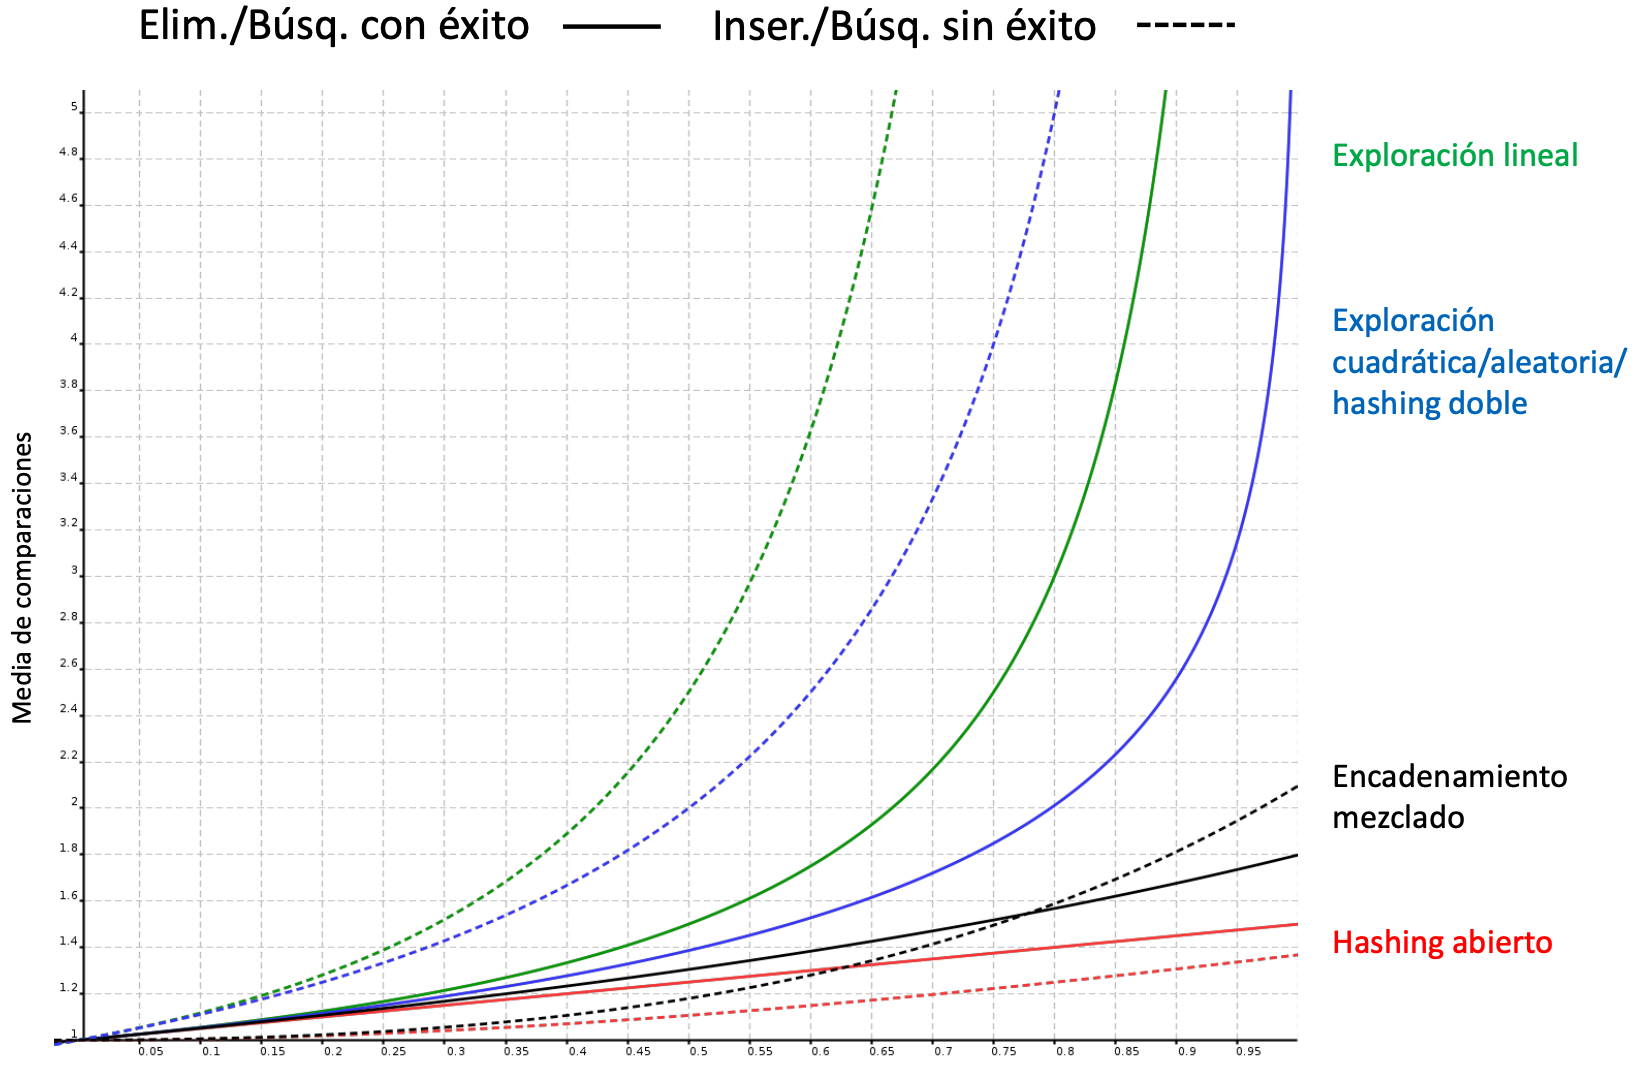
\includegraphics[width=.9\textwidth]{assets/hash1.png}
  \end{center}
  \caption{Gráfica comparativa entre diferentes tipos de hashing}
\end{figure}

\section{Redimensionamiento y Rehashing}
Cuando una tabla tiene un factor de carga alto, es decir, está muy llena, se realiza un \textbf{redimensionamiento} de la misma (se crea una tabla más grande y se reinsercionan de nuevo los elementos de la anterior) o un \textbf{rehashing} (se reinsercionan los elementos en la misma tabla para eliminar las casillas que están marcadas como borradas).

Esto hace que se restaure la eficiencia de la tabla.

\section{Comparación con árboles de búsqueda}
Sabemos que las tablas hash ofrecen un tiempo de búsqueda del orden \(O(1)\) si controlamos el facto de carga, pero un coste de \(O(n)\) para el peor caso.

Como vimos en el tema de árboles de búsqueda, estos ofrecen un tiempo de búsqueda del orden \(O(log\ n)\), con la ventaja de que estos árboles son dinámicos, es decir, no tenemos que prever el número máximo de elementos a almacenar.

Otra ventaja es que los \textbf{árboles de búsqueda} ofrecen un conjunto de operaciones más amplios, donde destaca el \textit{acceso a los elementos en orden}, gracias a esto podemos acceder los mínimos y máximos valores respecto a otro o buscar el minimo valor o máximo del árbol.

Como conclusión tenemos que si queremos realizar búsquedas rápidas la elección correcta es el uso de \textbf{tablas de dispersión o hash} cuando se elige una buena función hash y controlamos adecuadamente el factor de carga. Sin embargo, si necesitamos tener los elementos ordenados, haremos uso de un \textbf{árbol de búsqueda}.